\documentclass{standalone}
\usepackage{tikz}
\usetikzlibrary{patterns, positioning}


\begin{document}
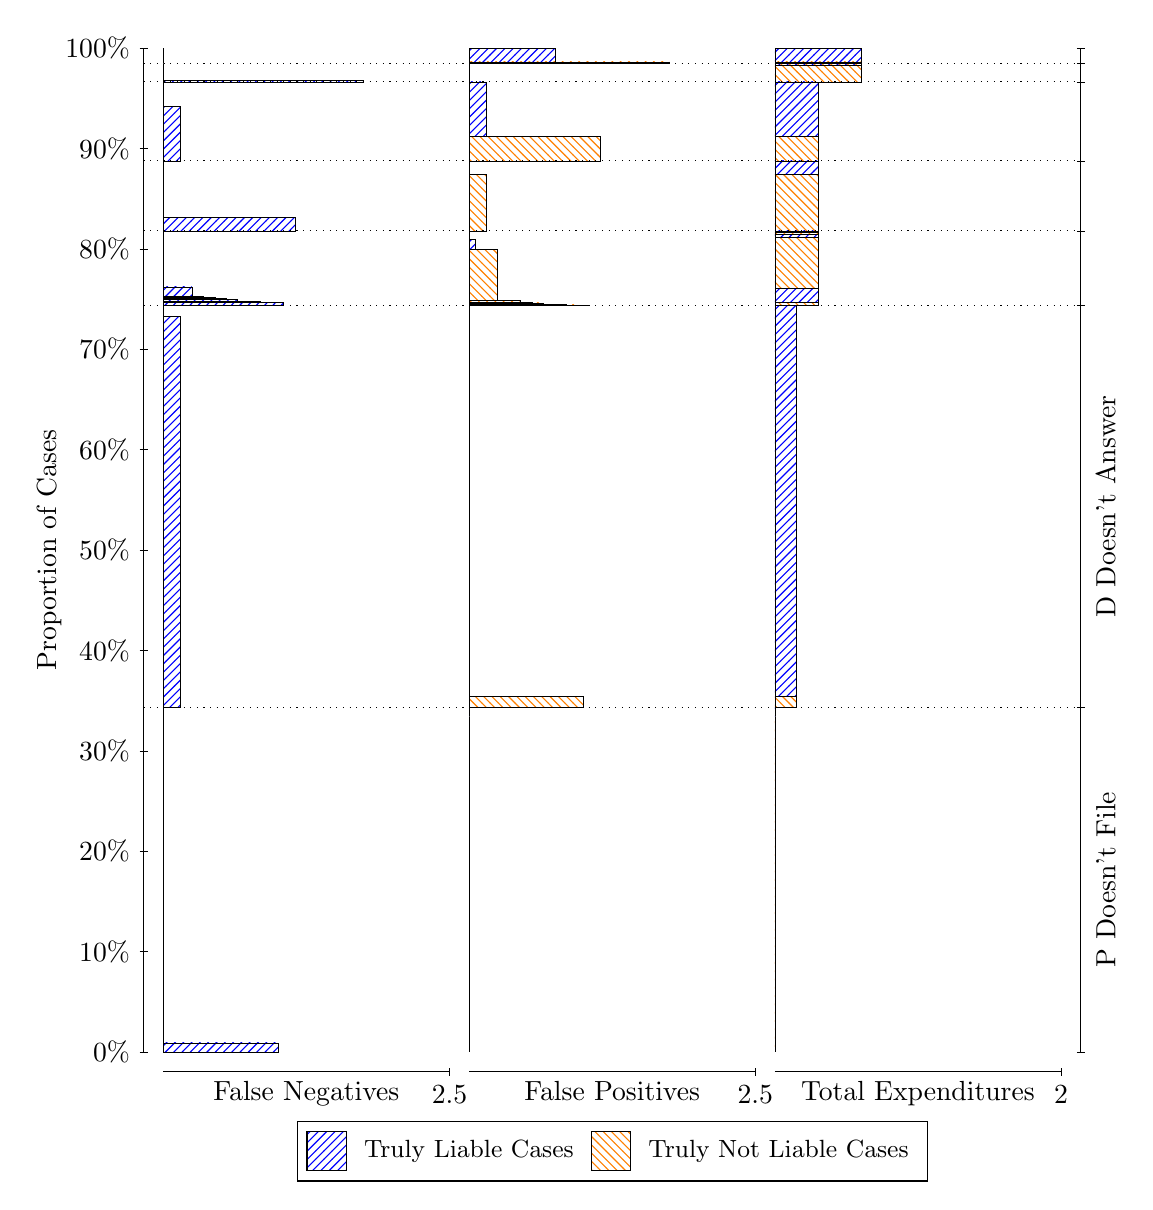
\begin{tikzpicture}
\draw[black, very thin] (1.5,1.75) -- (1.5,14.5);
\node[rotate=90, text=black, anchor=center] at (0.3, 8.125) {Proportion of Cases};
\draw[black, very thin] (1.45,1.75) -- (1.55,1.75);
\node[text=black, anchor=east] at (1.45, 1.75) {0\%};
\draw[black, very thin] (1.45,3.025) -- (1.55,3.025);
\node[text=black, anchor=east] at (1.45, 3.025) {10\%};
\draw[black, very thin] (1.45,4.3) -- (1.55,4.3);
\node[text=black, anchor=east] at (1.45, 4.3) {20\%};
\draw[black, very thin] (1.45,5.575) -- (1.55,5.575);
\node[text=black, anchor=east] at (1.45, 5.575) {30\%};
\draw[black, very thin] (1.45,6.85) -- (1.55,6.85);
\node[text=black, anchor=east] at (1.45, 6.85) {40\%};
\draw[black, very thin] (1.45,8.125) -- (1.55,8.125);
\node[text=black, anchor=east] at (1.45, 8.125) {50\%};
\draw[black, very thin] (1.45,9.4) -- (1.55,9.4);
\node[text=black, anchor=east] at (1.45, 9.4) {60\%};
\draw[black, very thin] (1.45,10.675) -- (1.55,10.675);
\node[text=black, anchor=east] at (1.45, 10.675) {70\%};
\draw[black, very thin] (1.45,11.95) -- (1.55,11.95);
\node[text=black, anchor=east] at (1.45, 11.95) {80\%};
\draw[black, very thin] (1.45,13.225) -- (1.55,13.225);
\node[text=black, anchor=east] at (1.45, 13.225) {90\%};
\draw[black, very thin] (1.45,14.5) -- (1.55,14.5);
\node[text=black, anchor=east] at (1.45, 14.5) {100\%};

\draw[black, very thin] (13.4,1.75) -- (13.4,14.5);
\draw[black, very thin] (13.35,1.75) -- (13.45,1.75);
\node[anchor=west] at (13.35, 1.75) {};
\draw[black, very thin] (13.35,6.1244) -- (13.45,6.1244);
\node[anchor=west] at (13.35, 6.1244) {};
\draw[black, very thin] (13.35,11.231) -- (13.45,11.231);
\node[anchor=west] at (13.35, 11.231) {};
\draw[black, very thin] (13.35,12.178) -- (13.45,12.178);
\node[anchor=west] at (13.35, 12.178) {};
\draw[black, very thin] (13.35,13.066) -- (13.45,13.066);
\node[anchor=west] at (13.35, 13.066) {};
\draw[black, very thin] (13.35,14.071) -- (13.45,14.071);
\node[anchor=west] at (13.35, 14.071) {};
\draw[black, very thin] (13.35,14.304) -- (13.45,14.304);
\node[anchor=west] at (13.35, 14.304) {};
\draw[black, very thin] (13.35,14.5) -- (13.45,14.5);
\node[anchor=west] at (13.35, 14.5) {};

\draw[black, very thin, pattern color=blue, pattern=north east lines] (1.75,1.75) rectangle (3.2033,1.8657);
\draw[black, very thin, pattern color=orange, pattern=north west lines] (1.75,1.8657) rectangle (1.75,6.1244);
\draw[black, very thin, pattern color=blue, pattern=north east lines] (1.75,6.1244) rectangle (1.968,11.087);
\draw[black, very thin, pattern color=orange, pattern=north west lines] (1.75,11.087) rectangle (1.75,11.231);
\draw[black, very thin, pattern color=blue, pattern=north east lines] (1.75,11.231) rectangle (3.276,11.266);
\draw[black, very thin, pattern color=blue, pattern=north east lines] (1.75,11.266) rectangle (3.1307,11.269);
\draw[black, very thin, pattern color=blue, pattern=north east lines] (1.75,11.269) rectangle (2.9853,11.279);
\draw[black, very thin, pattern color=blue, pattern=north east lines] (1.75,11.279) rectangle (2.84,11.285);
\draw[black, very thin, pattern color=blue, pattern=north east lines] (1.75,11.285) rectangle (2.6947,11.31);
\draw[black, very thin, pattern color=blue, pattern=north east lines] (1.75,11.31) rectangle (2.5493,11.318);
\draw[black, very thin, pattern color=blue, pattern=north east lines] (1.75,11.318) rectangle (2.404,11.333);
\draw[black, very thin, pattern color=blue, pattern=north east lines] (1.75,11.333) rectangle (2.2587,11.343);
\draw[black, very thin, pattern color=blue, pattern=north east lines] (1.75,11.343) rectangle (2.1133,11.467);
\draw[black, very thin, pattern color=orange, pattern=north west lines] (1.75,11.467) rectangle (1.75,12.178);
\draw[black, very thin, pattern color=blue, pattern=north east lines] (1.75,12.178) rectangle (3.4213,12.353);
\draw[black, very thin, pattern color=orange, pattern=north west lines] (1.75,12.353) rectangle (1.75,13.066);
\draw[black, very thin, pattern color=blue, pattern=north east lines] (1.75,13.066) rectangle (1.968,13.759);
\draw[black, very thin, pattern color=orange, pattern=north west lines] (1.75,13.759) rectangle (1.75,14.071);
\draw[black, very thin, pattern color=blue, pattern=north east lines] (1.75,14.071) rectangle (4.2933,14.089);
\draw[black, very thin, pattern color=orange, pattern=north west lines] (1.75,14.089) rectangle (1.75,14.304);
\draw[black, very thin, pattern color=orange, pattern=north west lines] (1.75,14.304) rectangle (1.75,14.325);
\draw[black, very thin, pattern color=blue, pattern=north east lines] (1.75,14.325) rectangle (1.75,14.5);
\draw[black, very thin, pattern color=orange, pattern=north west lines] (5.6333,1.75) rectangle (5.6333,6.0087);
\draw[black, very thin, pattern color=blue, pattern=north east lines] (5.6333,6.0087) rectangle (5.6333,6.1244);
\draw[black, very thin, pattern color=orange, pattern=north west lines] (5.6333,6.1244) rectangle (7.0867,6.2682);
\draw[black, very thin, pattern color=blue, pattern=north east lines] (5.6333,6.2682) rectangle (5.6333,11.231);
\draw[black, very thin, pattern color=orange, pattern=north west lines] (5.6333,11.231) rectangle (7.1593,11.236);
\draw[black, very thin, pattern color=orange, pattern=north west lines] (5.6333,11.236) rectangle (7.014,11.238);
\draw[black, very thin, pattern color=orange, pattern=north west lines] (5.6333,11.238) rectangle (6.8687,11.241);
\draw[black, very thin, pattern color=orange, pattern=north west lines] (5.6333,11.241) rectangle (6.7233,11.242);
\draw[black, very thin, pattern color=orange, pattern=north west lines] (5.6333,11.242) rectangle (6.578,11.262);
\draw[black, very thin, pattern color=orange, pattern=north west lines] (5.6333,11.262) rectangle (6.4327,11.266);
\draw[black, very thin, pattern color=orange, pattern=north west lines] (5.6333,11.266) rectangle (6.4327,11.268);
\draw[black, very thin, pattern color=orange, pattern=north west lines] (5.6333,11.268) rectangle (6.2873,11.297);
\draw[black, very thin, pattern color=orange, pattern=north west lines] (5.6333,11.297) rectangle (6.142,11.298);
\draw[black, very thin, pattern color=orange, pattern=north west lines] (5.6333,11.298) rectangle (5.9967,11.942);
\draw[black, very thin, pattern color=blue, pattern=north east lines] (5.6333,11.942) rectangle (5.706,12.067);
\draw[black, very thin, pattern color=blue, pattern=north east lines] (5.6333,12.067) rectangle (5.6333,12.178);
\draw[black, very thin, pattern color=orange, pattern=north west lines] (5.6333,12.178) rectangle (5.8513,12.892);
\draw[black, very thin, pattern color=blue, pattern=north east lines] (5.6333,12.892) rectangle (5.6333,13.066);
\draw[black, very thin, pattern color=orange, pattern=north west lines] (5.6333,13.066) rectangle (7.3047,13.378);
\draw[black, very thin, pattern color=blue, pattern=north east lines] (5.6333,13.378) rectangle (5.8513,14.071);
\draw[black, very thin, pattern color=orange, pattern=north west lines] (5.6333,14.071) rectangle (5.6333,14.286);
\draw[black, very thin, pattern color=blue, pattern=north east lines] (5.6333,14.286) rectangle (5.6333,14.304);
\draw[black, very thin, pattern color=orange, pattern=north west lines] (5.6333,14.304) rectangle (8.1767,14.325);
\draw[black, very thin, pattern color=blue, pattern=north east lines] (5.6333,14.325) rectangle (6.7233,14.5);
\draw[black, very thin, pattern color=orange, pattern=north west lines] (9.5167,1.75) rectangle (9.5167,6.0087);
\draw[black, very thin, pattern color=blue, pattern=north east lines] (9.5167,6.0087) rectangle (9.5167,6.1244);
\draw[black, very thin, pattern color=orange, pattern=north west lines] (9.5167,6.1244) rectangle (9.7892,6.2682);
\draw[black, very thin, pattern color=blue, pattern=north east lines] (9.5167,6.2682) rectangle (9.7892,11.231);
\draw[black, very thin, pattern color=orange, pattern=north west lines] (9.5167,11.231) rectangle (10.062,11.266);
\draw[black, very thin, pattern color=blue, pattern=north east lines] (9.5167,11.266) rectangle (10.062,11.452);
\draw[black, very thin, pattern color=orange, pattern=north west lines] (9.5167,11.452) rectangle (10.062,12.096);
\draw[black, very thin, pattern color=blue, pattern=north east lines] (9.5167,12.096) rectangle (10.062,12.131);
\draw[black, very thin, pattern color=orange, pattern=north west lines] (9.5167,12.131) rectangle (10.062,12.163);
\draw[black, very thin, pattern color=blue, pattern=north east lines] (9.5167,12.163) rectangle (10.062,12.178);
\draw[black, very thin, pattern color=orange, pattern=north west lines] (9.5167,12.178) rectangle (10.062,12.892);
\draw[black, very thin, pattern color=blue, pattern=north east lines] (9.5167,12.892) rectangle (10.062,13.066);
\draw[black, very thin, pattern color=orange, pattern=north west lines] (9.5167,13.066) rectangle (10.062,13.378);
\draw[black, very thin, pattern color=blue, pattern=north east lines] (9.5167,13.378) rectangle (10.062,14.071);
\draw[black, very thin, pattern color=orange, pattern=north west lines] (9.5167,14.071) rectangle (10.607,14.286);
\draw[black, very thin, pattern color=blue, pattern=north east lines] (9.5167,14.286) rectangle (10.607,14.304);
\draw[black, very thin, pattern color=orange, pattern=north west lines] (9.5167,14.304) rectangle (10.607,14.325);
\draw[black, very thin, pattern color=blue, pattern=north east lines] (9.5167,14.325) rectangle (10.607,14.5);
\draw[black, dotted] (1.5,6.1244) -- (13.4,6.1244);
\draw[black, dotted] (1.5,11.231) -- (13.4,11.231);
\draw[black, dotted] (1.5,12.178) -- (13.4,12.178);
\draw[black, dotted] (1.5,13.066) -- (13.4,13.066);
\draw[black, dotted] (1.5,14.071) -- (13.4,14.071);
\draw[black, dotted] (1.5,14.304) -- (13.4,14.304);
\draw[black, very thin] (1.75,1.5) -- (5.3833,1.5);
\node[text=black, anchor=north] at (3.5667, 1.5) {False Negatives};
\draw[black, very thin] (5.3833,1.45) -- (5.3833,1.55);
\node[text=black, anchor=north] at (5.3833, 1.45) {2.5};

\draw[black, very thin] (5.6333,1.5) -- (9.2667,1.5);
\node[text=black, anchor=north] at (7.45, 1.5) {False Positives};
\draw[black, very thin] (9.2667,1.45) -- (9.2667,1.55);
\node[text=black, anchor=north] at (9.2667, 1.45) {2.5};

\draw[black, very thin] (9.5167,1.5) -- (13.15,1.5);
\node[text=black, anchor=north] at (11.333, 1.5) {Total Expenditures};
\draw[black, very thin] (13.15,1.45) -- (13.15,1.55);
\node[text=black, anchor=north] at (13.15, 1.45) {2};

\node[text=black, centered, rotate=90] at (13.72, 3.9372) {P Doesn't File};
\node[text=black, centered, rotate=90] at (13.72, 8.6778) {D Doesn't Answer};






\draw (7.449999999999999,1.5) node[draw=none] (baseCoordinate) {};
\begin{scope}[align=center]
        \matrix[scale=0.5, draw=black, below=0.5cm of baseCoordinate, nodes={draw}, column sep=0.1cm]{
            \node[rectangle, draw, minimum width=0.5cm, minimum height=0.5cm, pattern color=blue, pattern=north east lines] {}; &
            \node[draw=none, font=\small, text=black] (B) {Truly Liable Cases}; &
            \node[rectangle, draw, minimum width=0.5cm, minimum height=0.5cm, pattern color=orange, pattern=north west lines] {}; &
            \node[draw=none, font=\small, text=black] (B) {Truly Not Liable Cases}; \\
            };
\end{scope}

\end{tikzpicture}
\end{document}